\documentclass[aspectratio=1610]{beamer}

\providecommand{\oritoneexamplemode}{light}
\usetheme[mode=\oritoneexamplemode,accent=blue]{Oritone}

\usepackage{pgfplots}
\pgfplotsset{compat=1.18, compat/show suggested version=false}
\oritonepgfplotssetup

\title[Oritone Example]{A Complete Oritone Deck}
\subtitle{Technical presentation defaults}
\author[A. Sterling]{Ada Sterling}
\coauthors{Benoit Sample and Clara Rivera}
\institute[Example Lab]{Example Laboratory for Reusable Documents}
\date{\today}

\biglogo{example-image-a}
\smalllogo{example-image-b}

\newcommand{\modeswatch}[2]{%
  \begin{tikzpicture}[baseline=-0.6ex]
    \draw[draw=divider, fill=#1] (0,0) rectangle (0.38,0.22);
  \end{tikzpicture}\enspace #2%
}

\begin{document}
\maketitle

\sectionframe{Overview}

\begin{frame}{Motivation}
  \begin{itemize}
    \item Shared colors, fonts, listings, and plot defaults.
    \item Compact title, footer, section, and closing frames.
    \item Regular, example, and alert blocks for technical talks.
    \item Light, dark, white, and black modes with selectable accent colors.
  \end{itemize}
\end{frame}

\begin{frame}{Mode and Accent Surface}
  \begin{columns}[T,totalwidth=\textwidth]
    \begin{column}{0.47\textwidth}
      \begin{block}{Document Modes}
        \modeswatch{background}{current background}\\[1mm]
        \modeswatch{foreground}{current foreground}\\[1mm]
        \modeswatch{surface}{surface}\\[1mm]
        \modeswatch{surface-raised}{raised surface}
      \end{block}
    \end{column}
    \begin{column}{0.47\textwidth}
      \begin{exampleblock}{Semantic Roles}
        \textcolor{success}{success text}\\
        \textcolor{warning}{warning text}\\
        \textcolor{danger}{danger text}\\
        \textcolor{info}{information text}
      \end{exampleblock}
    \end{column}
  \end{columns}
\end{frame}

\begin{frame}{Blocks}
  \begin{block}{Regular Block}
    Use regular blocks for definitions, assumptions, and central claims. The
    block rule follows the selected accent family.
  \end{block}
  \begin{exampleblock}{Example Block}
    Example blocks use the success role and work well for observations or
    verified results.
  \end{exampleblock}
  \begin{alertblock}{Alert Block}
    Alert blocks use the danger role for caveats, failed checks, and required
    action.
  \end{alertblock}
\end{frame}

\begin{frame}{Lists and Emphasis}
  \begin{columns}[T,totalwidth=\textwidth]
    \begin{column}{0.48\textwidth}
      \begin{itemize}
        \item First-level item with the theme marker.
        \item Nested evidence:
          \begin{itemize}
            \item Compact second-level marker.
            \item Short supporting point.
          \end{itemize}
        \item \alert{Alert text} keeps warnings visible.
      \end{itemize}
    \end{column}
    \begin{column}{0.48\textwidth}
      \begin{enumerate}
        \item Define the model.
        \item Run the workflow.
        \item Check diagnostics.
        \item Archive artifacts.
      \end{enumerate}
    \end{column}
  \end{columns}
\end{frame}

\sectionframe{Technical Content}

\begin{frame}{Mathematics}
  A compact objective can be written as
  \begin{equation*}
    \mathcal{J}(u,\theta)
    =
    \frac{1}{2}\lVert G(u)-y\rVert_{\Gamma^{-1}}^2
    + \lambda \int_\Omega
      \frac{1}{2}\lvert\nabla u\rvert^2 + V(u,\theta)\,\mathrm{d}x .
  \end{equation*}
  The surrounding text uses the same font choices as the document classes:
  Roboto Condensed, STIX Two serif and math, and Recursive Mono.
\end{frame}

\begin{frame}{Table}
  \begin{table}
    \centering
    \caption{A compact solver summary.}
    \begin{tabular}{lrr}
      \hline
      Case & Iterations & Relative error \\
      \hline
      Coarse & 18 & \(2.4\times10^{-2}\) \\
      Medium & 27 & \(6.1\times10^{-3}\) \\
      Fine & 41 & \(1.5\times10^{-3}\) \\
      Validation & 39 & \(1.8\times10^{-3}\) \\
      \hline
    \end{tabular}
  \end{table}
\end{frame}

\begin{frame}{Plot}
  \begin{center}
    \begin{tikzpicture}
      \begin{axis}[
        width=0.86\textwidth,
        height=0.55\textheight,
        xlabel={Refinement level},
        ylabel={Relative error},
        ymode=log,
        grid=major,
        legend pos=south west
      ]
        \addplot coordinates {(1,1.83e-1) (2,4.61e-2) (3,1.16e-2) (4,2.90e-3)};
        \addlegendentry{standard}
        \addplot coordinates {(1,2.40e-1) (2,7.20e-2) (3,2.20e-2) (4,6.90e-3)};
        \addlegendentry{stabilized}
      \end{axis}
    \end{tikzpicture}
  \end{center}
\end{frame}

\begin{frame}[fragile]{Code}
\begin{lstlisting}[language=Julia]
function residual(values)
  total = 0.0
  for value in values
    total += abs(value)
  end
  return total
end
\end{lstlisting}
\end{frame}

\sectionframe{Visual Slides}

\slidebackground{example-image}
\begin{frame}{Image-backed Slide}
  \begin{columns}[T,totalwidth=\textwidth]
    \begin{column}{0.52\textwidth}
      The theme can place a contextual image into the curved upper-right
      background area while preserving readable text and the normal footer.
    \end{column}
    \begin{column}{0.38\textwidth}
      \begin{block}{Use Cases}
        product shots, instruments, maps, facilities, or experiment photos.
      \end{block}
    \end{column}
  \end{columns}
\end{frame}
\noslidebackground

\standoutframe{%
  \vfill
  {\usebeamerfont{sectionframetitle}\usebeamercolor[fg]{sectionframetitle}
  Standout frames}\\[4mm]
  {\usebeamerfont{normal text}
  Use these for section breaks, quotes, or a single high-signal statement.}
  \vfill
}

\begin{frame}{References and Links}
  \begin{thebibliography}{9}
    \bibitem{demo}
      A. Sterling and B. Sample.
      \newblock Reusable presentation systems for technical teams.
      \newblock Example Workshop, 2026.
  \end{thebibliography}

  \vspace{3mm}
  Project page: \weblink{example.com/oritone}
\end{frame}

\closingframe{Thank you}{\weblink{example.com/oritone}}{Questions}

\end{document}
